\documentclass[polish,10pt]{article}
\usepackage[T1]{fontenc}
   	\usepackage{polski}
    \usepackage{babel}
	\usepackage{subfigure}
	\usepackage{graphicx}
	\usepackage{geometry}
	\usepackage{listings}
	\usepackage{float}
    \usepackage{graphicx}
    \usepackage{listings}
    \renewcommand{\lstlistlistingname}{Spis listingów}
    \renewcommand{\listfigurename}{WYKAZ RYSUNKÓW}
    \renewcommand{\listtablename}{WYKAZ TABEL}
 
    \usepackage[backend=biber, style=numeric, bibstyle=ieee,
            sorting=none, isbn=false, urldate=ymd,
            doi=false, url=true]{biblatex}
    \addbibresource{bibliography/bibliography.bib}
    \renewbibmacro{in:}{}
    \renewcommand*{\bibfont}{\small}
    \newcommand{\bibliographyname}{WYKAZ LITERATURY}


    \usepackage[unicode=true]{hyperref}

\title{Testowanie na podstawie właściwości}
\author{inż. Paulina Brzęcka 184701 \and inż. Marek Borzyszkowski 184266}
\date{\today}
\begin{document}

\pgtitleframe

\section{Wstęp}
Istnieje wiele koncepcji testowania oprogramowania, jedną z nich jest testowanie na podstawie właściwości \cite{pbt_bib}.
Ten dokument ma na celu ukazanie:
\begin{enumerate}
  \item na czym polega testowanie na podstawie właściwości.
  \item Czym różni się ono od klasycznego podejścia do testowania.
  \item Jakie są strategie testowania na podstawie właściwości. 
  \item Jak przy wykorzystaniu konceptu QuickCheck znaleźć wartości początkowe nieprzechodzące testy.
\end{enumerate}

\begin{frame}{Przykład}
    TODO
\end{frame}

\section{Strategie}

Testowanie na podstawie właściwości nie jest proste w zastosowaniu, przynajmniej przy pierwszej próbie.
Istnieją jednak pewne schematy wskazujące drogę, jak stworzyć takie testy.
\subsection{Różne ścieżki, ten sam wynik}

Jedną z podstawowych strategii skorzystanie z komutatywności niektórych operacji. Można to zrobić poprzez wykonanie operacji w różnej kolejności, jak zaprezentowano w \refrys{fig:commutative_strategy}.
\begin{figure}[h]
    \centering
    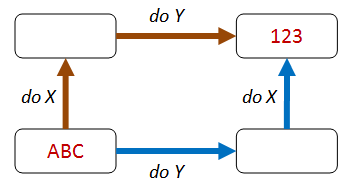
\includegraphics[width=0.5\textwidth]{images/property_commutative.png}
    \caption{Strategia - komutatywność}
    \label{fig:commutative_strategy}
\end{figure}

Przykładem takiej strategii może być komutatywność dodawania z \reflist{kod:add_all_properties}, gdzie wykorzystano \texttt{add x y}, jak i odwrotność tej operacji \texttt{add y x}. 
Innym przykładem jest test metody \texttt{sort} danej listy. 
Wykonanie sortowania, a następnie dodanie do każdego elementu listy \texttt{1} powinno dać taki sam efekt jak dodanie \texttt{1} do każdego z elementów listy, a następnie jej posortowanie \refrys{fig:commutative_strategy_list_sort} \reflist{kod:list_sort_add1}.

\begin{figure}
    \centering
    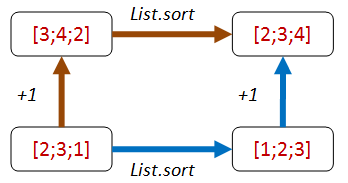
\includegraphics[width=0.5\textwidth]{images/property_list_sort1.png}
    \caption{Strategia - komutatywność - sortowanie listy}
    \label{fig:commutative_strategy_list_sort}
\end{figure}
\lstset{language=FSharp, basicstyle=\scriptsize}
\begin{lstlisting}[frame=single,caption={Test sortowania listy z wykorzystaniem strategii komutatywnej},label=kod:list_sort_add1]
    let addThenSort_eq_sortThenAdd sortFn aList =
        let add1 x = x + 1

        let result1 = aList |> sortFn |> List.map add1
        let result2 = aList |> List.map add1 |> sortFn
        result1 = result2
\end{lstlisting}

\subsection{Tam i z powrotem}

Test z wykorzystaniem inwersji \refrys{fig:inverse_strategy}, polega na sprawdzeniu, czy po zaaplikowaniu testowanej funkcji, następnie wykorzystaniu funkcji odwrotnej do otrzymania początkowych wartości.   
\begin{figure}
    \centering
    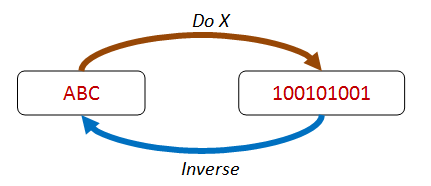
\includegraphics[width=0.5\textwidth]{images/property_inverse.png}
    \caption{Strategia - inwersja}
    \label{fig:inverse_strategy}
\end{figure}
Przykładem takiego testu mogą być przeciwne operacje matematyczne jak:
\begin{itemize}
    \item \texttt{dodawanie/odejmowanie}
    \item \texttt{mnożenie/dzielenie}
    \item \texttt{potęga/logarytm}.
\end{itemize} 
Innymi przykładami są operacje niekoniecznie matematyczne:
\begin{itemize}
    \item \texttt{serializacja/deserializacja}
    \item \texttt{zapis/odczyt z pliku}
    \item \texttt{wstaw/sprawdź czy zawiera}.
    \item \texttt{odwrócenie listy/odwrócenie listy}
\end{itemize} 

\subsection{Są rzeczy niezmienne}

Czasami testowana funkcja przetwarzając dane zachowuje część ich właściwości \refrys{fig:invariant_strategy}. Chociażby funkcje \texttt{sort} lub \texttt{map} wykonane na liście \texttt{n} elementów, zwracaja odpowiednio zmodyfikowaną listę \texttt{n} elementową.

\begin{figure}
    \centering
    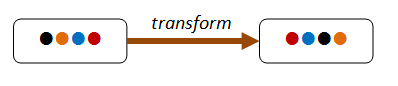
\includegraphics[width=0.5\textwidth]{images/property_invariant.png}
    \caption{Strategia - niezmienność}
    \label{fig:invariant_strategy}
\end{figure}

\subsection{Z czasem rzeczy przestają się zmieniać}

Inną właściwością funkcji może być niezmienność wyniku funkcji po ponownym jej zaaplikowaniu \refrys{fig:independance_strategy}. Innymi słowy, wykonanie funkcji 2 razy daje taki sam efekt, jak jednokrotne jej zaaplikowanie.

\begin{figure}
    \centering
    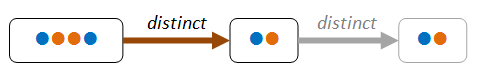
\includegraphics[width=0.5\textwidth]{images/property_idempotence.png}
    \caption{Strategia - idempotentność}
    \label{fig:independance_strategy}
\end{figure}

Przykładami takich operacji, dla których taki typ testu miałby zastosowanie to metoda \texttt{distinct} wykonana na danej liście, lub wykonanie \texttt{update} na danej bazie danych.

\subsection{Dziel i rządź}

Istnieją sposoby na testowanie na podstawie właściwości jest wykorzystanie rekursywności struktur przekazywanych do funkcji, takich jak \texttt{listy}, \texttt{drzewa} \refrys{fig:recursive_strategy}. Przykładem może być sprawdzenie za pomocą tej metody funkcji sort \reflist{kod:list_sort_rec}.

\begin{figure}
    \centering
    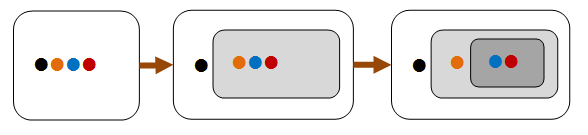
\includegraphics[width=0.5\textwidth]{images/property_induction.png}
    \caption{Strategia - rekursywność}
    \label{fig:recursive_strategy}
\end{figure}

\lstset{language=FSharp, basicstyle=\scriptsize}
\begin{lstlisting}[frame=single,caption={Test sortowania listy z wykorzystaniem strategii rekursywnej},label=kod:list_sort_rec]
let rec firstLessThanSecond_andTailIsSorted sortFn (aList:int list) =
  let sortedList = aList |> sortFn
  match sortedList with
  | [] -> true
  | [first] -> true
  | [first;second] -> first <= second
  | first::second::rest->
    first <= second &&
    let tail = second::rest
    // check that tail is sorted
    firstLessThanSecond_andTailIsSorted sortFn tail
\end{lstlisting}

\subsection{Łatwiej zweryfikować niż zaimplementować}
Niekiedy testowana funkcja jest skomplikowana, ale jej rezultat da się łatwo sprawdzić. Przykładem może być funkcja wyszukująca wyjście z labiryntu \refrys{fig:easy_verification_strategy}, gdzie sam algorytm wyszukiwania odpowiedniej ścieżki jest skomplikowany, 
natomiast samo sprawdzenie, czy ścieżka dobrze prowadzi do wyjścia można w łatwy sposób zweryfikować.

\begin{figure}
    \centering
    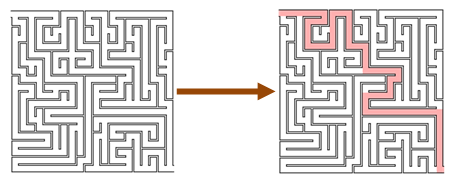
\includegraphics[width=0.5\textwidth]{images/property_easy_verification.png}
    \caption{Strategia - łatwe sprawdzenie}
    \label{fig:easy_verification_strategy}
\end{figure}

\subsection{Testowanie z wyrocznią}

\section{QuickCheck}
QuickCheck został stworzony w języku Haskell jako pierwsze narzędzie wspierające testowanie oparte na właściwościach. Jest on inspiracją dla bibliotek w innych językach, takich jak FsCheck dla .NET.

\subsection{Cechy QuickCheck}
\begin{itemize}
    \item Automatyczne generowanie danych testowych.
    \item Sprawdzanie, czy zdefiniowane właściwości funkcji są spełniane dla wielu losowych przypadków.
    \item W przypadku wykrycia błędu narzędzie redukuje (\textit{shrinking}) dane wejściowe, aby znaleźć minimalny przykład prowadzący do błędu.
\end{itemize}

\begin{figure}[h]
    \centering
    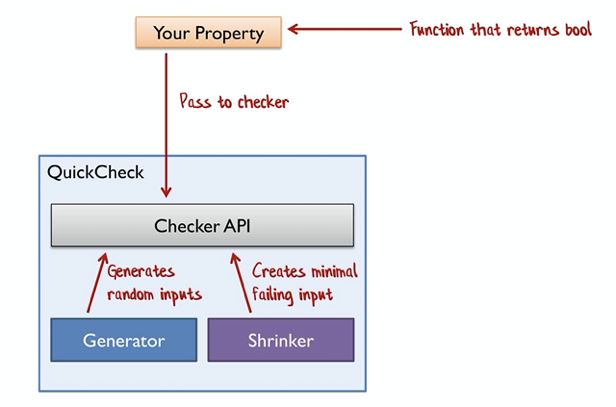
\includegraphics[width=0.8\textwidth]{images/schema.png}
    \caption{Schemat działania QuickCheck}
\end{figure}

\subsection{Działanie}
\begin{enumerate}
    \item \textbf{Checker API} wykrywa typ wejścia funkcji.
    \item Wywoływany jest generator odpowiedniego typu.
    \item Następuje generowanie przypadków testowych.
    \item Przypadki testowe są przekazywane do testowanej właściwości.
\end{enumerate}

\subsection{Funkcje}
\begin{itemize}
    \item \textbf{Check.Quick} -- uruchamia szybki test, sprawdzając właściwość dla domyślnej liczby losowych przypadków (np. 100).
    \item \textbf{Check.Verbose} -- działa jak Check.Quick, ale wyświetla więcej szczegółowych informacji o danych testowych.
    \item \textbf{Generowanie danych wejściowych} -- FsCheck wspiera generowanie danych dla typów prostych (np. \texttt{int}, \texttt{float}, \texttt{string}) i bardziej złożonych struktur, takich jak listy czy rekordy.
\end{itemize}

\subsection{Pisanie właściwości w FsCheck}

FsCheck umożliwia definiowanie właściwości w formie funkcji logicznych. Właściwości opisują, jakie warunki zawsze muszą być spełnione przez funkcję.

Przykład: Odwracanie listy
Dla funkcji \texttt{reverse}, która odwraca listę, możemy zdefiniować właściwość:
\begin{itemize}
    \item Odwrócenie listy dwukrotnie powinno zwrócić pierwotną listę.
\end{itemize}

\lstset{language=FSharp, basicstyle=\scriptsize}
\begin{lstlisting}[frame=single,caption={Definicja właściwości dla odwracania listy},label=kod:listingA]
let reverseProperty (xs: int list) =
    List.rev (List.rev xs) = xs

Check.Quick reverseProperty
\end{lstlisting}

\subsection{Generacja danych testowych}

FsCheck pozwala na tworzenie własnych generatorów danych wybranego typu. Jest to przydatne, gdy chcemy testować funkcję na specyficznych danych. \\
Na początku tworzymy generator, następnie generujemy dane testowe podając maksymalny rozmiar przypadku testowego (w przypadku stuktur danych) oraz liczbę przypadków testowych.\\
Zarówno przy generowaniu danych testowych, jak i przy późniejszej redukcji danych (shrinking) wykorzystywany jest arbitraż (Arb).\\
Jest to mechanizm definiowania sposobu generowania losowych danych dla konkretnego typu. Dzięki arbitrażowi można dostosować sposób generowania danych, wprowadzić dodatkowe ograniczenia, a nawet zdefiniować własne typy i ich generatory.

\lstset{language=FSharp, basicstyle=\scriptsize\ttfamily}
\begin{lstlisting}[frame=single,caption={Przykład generatora dla liczb dodatnich},label=kod:listingA]
let intGenerator = Arb.generate<int>
Gen.sample 100 3 intGenerator  // [-37; 24; -62]

// Przyklad generowania liczb dodatnich:
type PositiveInt = PositiveInt of int

let positiveIntGen =
    Gen.suchThat ((<) 0) Arb.generate<int>
Arb.register<PositiveInt>(positiveIntGen)

type Generators =
    static member PositiveInt() =
        Arb.fromGen positiveIntGen
Arb.register<Generators>() // rejestracja generatora by Quick.Check mogl zostac uzyty

let intListGenerator = Arb.generate<int list>
Gen.sample 5 10 intListGenerator 
// [ []; []; [-4]; [0; 3; -1; 2]; [1]; [1]; []; [0; 1; -2]; []; [-1; -2]]

let stringGenerator = Arb.generate<string>
Gen.sample 10 3 stringGenerator // [""; "eiX$a^"; "U%0Ika&r"]

type Point = {x:int; y:int; color: Color}
let pointGenerator = Arb.generate<Point>
Gen.sample 50 10 pointGenerator
(*
{x = -8; y = 12; color = Green -4;};
    {x = 28; y = -31; color = Green -6;};
    {x = 11; y = 27; color = Red;};
    {x = -2; y = -13; color = Red;};
    {x = 6; y = 12; color = Red;};
    // itd
*)
\end{lstlisting}

\subsection{Shrinking}

Po fazie generowania danych losowych dane wejściowe są ustawione od najmniejszej do największej wartości. Jeśli jakiekolwiek dane wejściowe spowodują, że właściwość przestanie być spełniona, narzędzie zaczyna "zmniejszać" pierwszy parametr, aby znaleźć mniejszą wartość. Dokładny proces zmniejszania zależy od typu danych (można go również nadpisać) \textit{(W przypadku liczb prowadząc do coraz mniejszych wartości.)}

\lstset{language=FSharp, basicstyle=\scriptsize}
\begin{lstlisting}[frame=single,caption={Przykład shrinking na liczbach},label=kod:listingA]
let isSmallerThan80 x = x < 80
isSmallerThan80 100 // false, so start shrinking

Arb.shrink 100 |> Seq.toList//  [0; 50; 75; 83; 94; 97; 99]
isSmallerThan80 0 // true
isSmallerThan80 50 // true
isSmallerThan80 75 // true
isSmallerThan80 83 // false, so shrink again

Arb.shrink 83 |> Seq.toList//  [0; 44; 66; 77; 80; 81]
isSmallerThan80 0 // true
isSmallerThan80 44 // true
isSmallerThan80 66 // true
isSmallerThan80 77 // true
isSmallerThan80 80 // false <- najmniejsza porazka
// wynik: Falsifiable, after 10 tests (2 shrinks)
\end{lstlisting}

Narzędzie jest bardzo przydatne do określenia, gdzie znajdują się granice błędów w testowaniu.\\
Shrink działa na customowych typach złożonych, dodatkowo można też generować własne sekwencje oraz zasady, w jaki sposób przeprowadzać customowe shrinkowanie. 

\lstset{language=FSharp, basicstyle=\scriptsize}
\begin{lstlisting}[frame=single,caption={Shrinkowanie ciągu znaków},label=kod:listingA]
Arb.shrink "abcd" |> Seq.toList
// ["bcd"; "acd"; "abd"; "abc"; "abca"; "abcb"; "abcc"; "abad"]
\end{lstlisting}

\subsection{Konfiguracja}
Czasem może zaistnieć potrzeba własnego dostosowania liczby testów itp. W tym celu można odpowiednio skonfigurować narzędzie:
\lstset{language=FSharp, basicstyle=\scriptsize}
\begin{lstlisting}[frame=single,caption={Dostosowanie konfiguracji testów},label=kod:listingA]
let config = {
    Config.Quick with
        MaxTest = 1000
    }
    Check.One(config,isSmallerThan80 )
    // result: Ok, passed 1000 tests. (a nie powinno :)
    
    let config = {
    Config.Quick with
        MaxTest = 10000
    }
    Check.One(config,isSmallerThan80 )
    // result: Falsifiable, after 8660 tests (1 shrink):
    //         80
\end{lstlisting}

\subsection{Warunki wstępne}
\lstset{language=FSharp, basicstyle=\scriptsize}
\begin{lstlisting}[frame=single,caption={Dodawanie warunków wstępnych},label=kod:listingA]
let preCondition x y =
    (x,y) <> (0,0)
    && (x,y) <> (2,2)

let additionIsNotMultiplication_withPreCondition x y =
preCondition x y ==> additionIsNotMultiplication x y
// Ok, passed 100 tests.
\end{lstlisting}

Jak widać, tego rodzaju rozwiązania mogą być użyte tylko w nielicznych przypadkach, gdy możemy zdefiniować niewielką liczbę "wyjątków od reguły".

\subsection{Testowanie kilku właściwości na raz}
W celu zapewnienia uporządkowania i ustrukturyzowania kodu istnieje możliwość testowania kilku właściwości równocześnie.
\lstset{language=FSharp, basicstyle=\scriptsize}
\begin{lstlisting}[frame=single,caption={Sprawdzanie wielu właściwości jednocześnie},label=kod:listingA]
type AdditionSpecification =
    static member ``Commutative`` x y =
      commutativeProperty x y
    static member ``Associative`` x y z =
      associativeProperty x y z
    static member ``Left Identity`` x =
      leftIdentityProperty x
    static member ``Right Identity`` x =
      rightIdentityProperty x
  
Check.QuickAll<AdditionSpecification>()

--- Checking AdditionSpecification ---
AdditionSpecification.Commutative-Ok, passed 100 tests.
AdditionSpecification.Associative-Ok, passed 100 tests.
AdditionSpecification.Left Identity-Ok, passed 100 tests.
AdditionSpecification.Right Identity-Ok, passed 100 tests.
\end{lstlisting}
\section{Podsumowanie}
TU JEST PODSUMOWANIE
\begin{frame}{Pytania}
    \begin{center}
        {\huge Pytania?}
    \end{center}
\end{frame}

\setbeamercovered{transparent}
\begin{frame}[allowframebreaks]{Bibliografia}
    \printbibliography
\end{frame}

\begin{frame}{Podziękowania}
    Chcielibyśmy podziękować Panu dr. inż. Janowi Cychnerskiemu za stworzenie 
    i udostępnienie stylu \href{https://github.com/jachoo/pg-beamer}{\emph{pg-beamer}}, 
    co zostało wykorzystane do stworzenia tej prezentacji.\\
    \url{https://github.com/jachoo/pg-beamer}
     
\end{frame}

\begin{frame}{Koniec}
    \begin{center}
        {\huge Dziękujemy za uwagę!}
    \end{center}
\end{frame}

\pglastframe

\end{document}